\addcontentsline{toc}{chapter}{Hardware}
\chapter{Hardware}

 
 
%%%%%%% INTRODUCTION %%%%%%
%\addcontentsline{toc}{section}{Introduction}
%\section{Introduction}
The advance in the computer vision discipline is greatly linked with the development in the hardware. The main components of a computer vision system are the following: 

\begin{itemize}
	\item{Power Supply: } Device needed by the other components in order to work. 
	\item{Acquisition device: } Device that captures the world and represents it as an array of data. That data can be two or three dimensional. 
	\item{Processing unit:} Receives the information from the acquisition device and processes it. It is usually programmable. Nowadays the most used processing units are PCs. 
	\item{I/O unit: } Serves as a bridge between the acquisition device and the processing unit if needed. 

\end{itemize}

In this chapter the state of the art of the different acquisition devices is going to be presented. 

%%%%%% ACQUISITION DEVICES %%%%%%
\addcontentsline{toc}{section}{Acquisition devices}
\section{Acquisition devices}
There are different acquisition devices being used in the computer vision field. They are usually classified depending on the output data they provide: 

\begin{itemize}
	\item{Cameras:}	The output data is two-dimensional. 
	\item{RGB-D sensors:} The output data is three-dimensional. 
\end{itemize}

The usage of one or another acquisition device depends on the application. The RGB-D sensors provide a higher number of information than the cameras. They reduce the ambiguities produced by the cameras when projecting the three-dimensional world into to dimensions. But also the RGB-D sensors output a higher amount of data. 
That is why, using three-dimensional information as the input of a software requires a higher-capacity processing unit than using two-dimensional data.



%%%%%% CAMERAS %%%%%%
%\addcontentsline{toc}{section}{Cameras}
%\section{Cameras}




%%%%%% RGB-D SENSORS %%%%%%
\addcontentsline{toc}{section}{RGB-D Sensors or Natural Interaction Devices}
\section{RGB-D Sensors or Natural Interaction Devices}

\addcontentsline{toc}{subsection}{History}
\subsection{History}

Computer vision is a field that needs specific hardware to retrieve a description of the world. This description has been done for a number of years in two dimensions. But this changed when the first version of an affordable RGB-D sensor appeared in 2010: the Kinect. This project uses a Kinect RGB-D sensor as the input of the system.
\\

This sensor was designed to be used in games, but developers soon realized the huge potential of the hardware for Computer Vision.  
Now, instead of a two-dimensional information as an input it was possible to have three-dimensional information. 
\\

The Microsoft corporation released the SDK (Software Development Kit) on June, 2011 \cite{kinectSDK}.
\\

But one year before, PrimeSense released their open source drivers and motion tracking middleware called NITE\cite{NITE}. 
PrimeSense is a company that manufactures RGB-D sensors and, in fact, the Kinect is based on their depth sensing reference. Hence, the software released by PrimeSense worked with the Kinect as well. 

From that time on, the OpenSource software related with the kinect has increased as well as the different models of RGB-D sensors available in the market.
In November 2010 OpenNI was created. Openni is an open-source software framework that can read the data from RGB-D sensors \cite{openni}.  

\addcontentsline{toc}{subsection}{How does the Kinect work?}
\subsection{How does the Kinect work?}
In this section the main components and functioning principles of the Kinect are going to be presented. Most of them are common with the other RGB-D sensors but others such as the VGA camera are optional, for example in some PrimeSense\cite{PrimeSense} models. 



\begin{figure}[h]
	\begin{center}
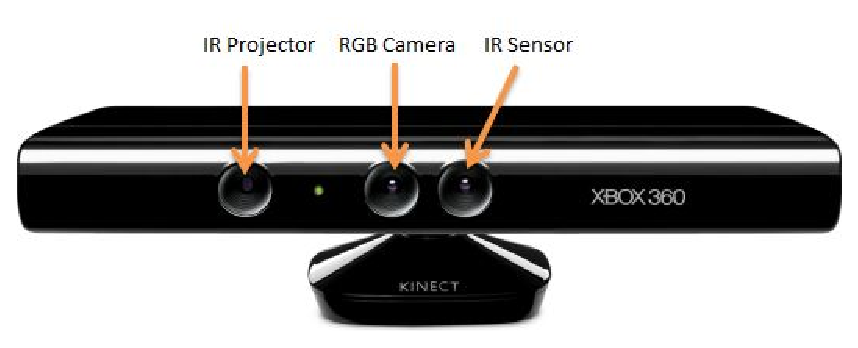
\includegraphics[scale=0.5]{img/kinect/kinect2.eps}
	\caption[Kinect Sensors]{Kinect sensors: depth sensor and VGA camera location.}
	\end{center}
\end{figure}


The parts that compose the Kinect sensor are the following: 

\begin{itemize}
	\item{VGA camera}\\
	The camera contained by the kinect has a pixel resolution of 640x480 and a frame rate of 30 fps. It is used mainly to provide the output data with the RGB components for each point. 
	
	\item{Depth sensor}\\
	The depth sensor consists on an infra-red projector combined with a monochrome CMOS sensor. This latter measures the time it takes the light to come back after being reflected on the objects. Knowing the speed of light it can be easily obtained the distance of the objects from the depth sensor. 

	\item{Multi-array microphone}\\
	This array of four microphones are included because the kinect was designed as a gaming device. They are not used for the three-dimensional world retrieving. 
	
	\item{Motorized tilt}\\
	This is another feature for games. It allows the kinect to follow the player's movements around the room. \cite{howkinectworks}
\end{itemize}



\begin{figure}[h]
	\begin{center}
	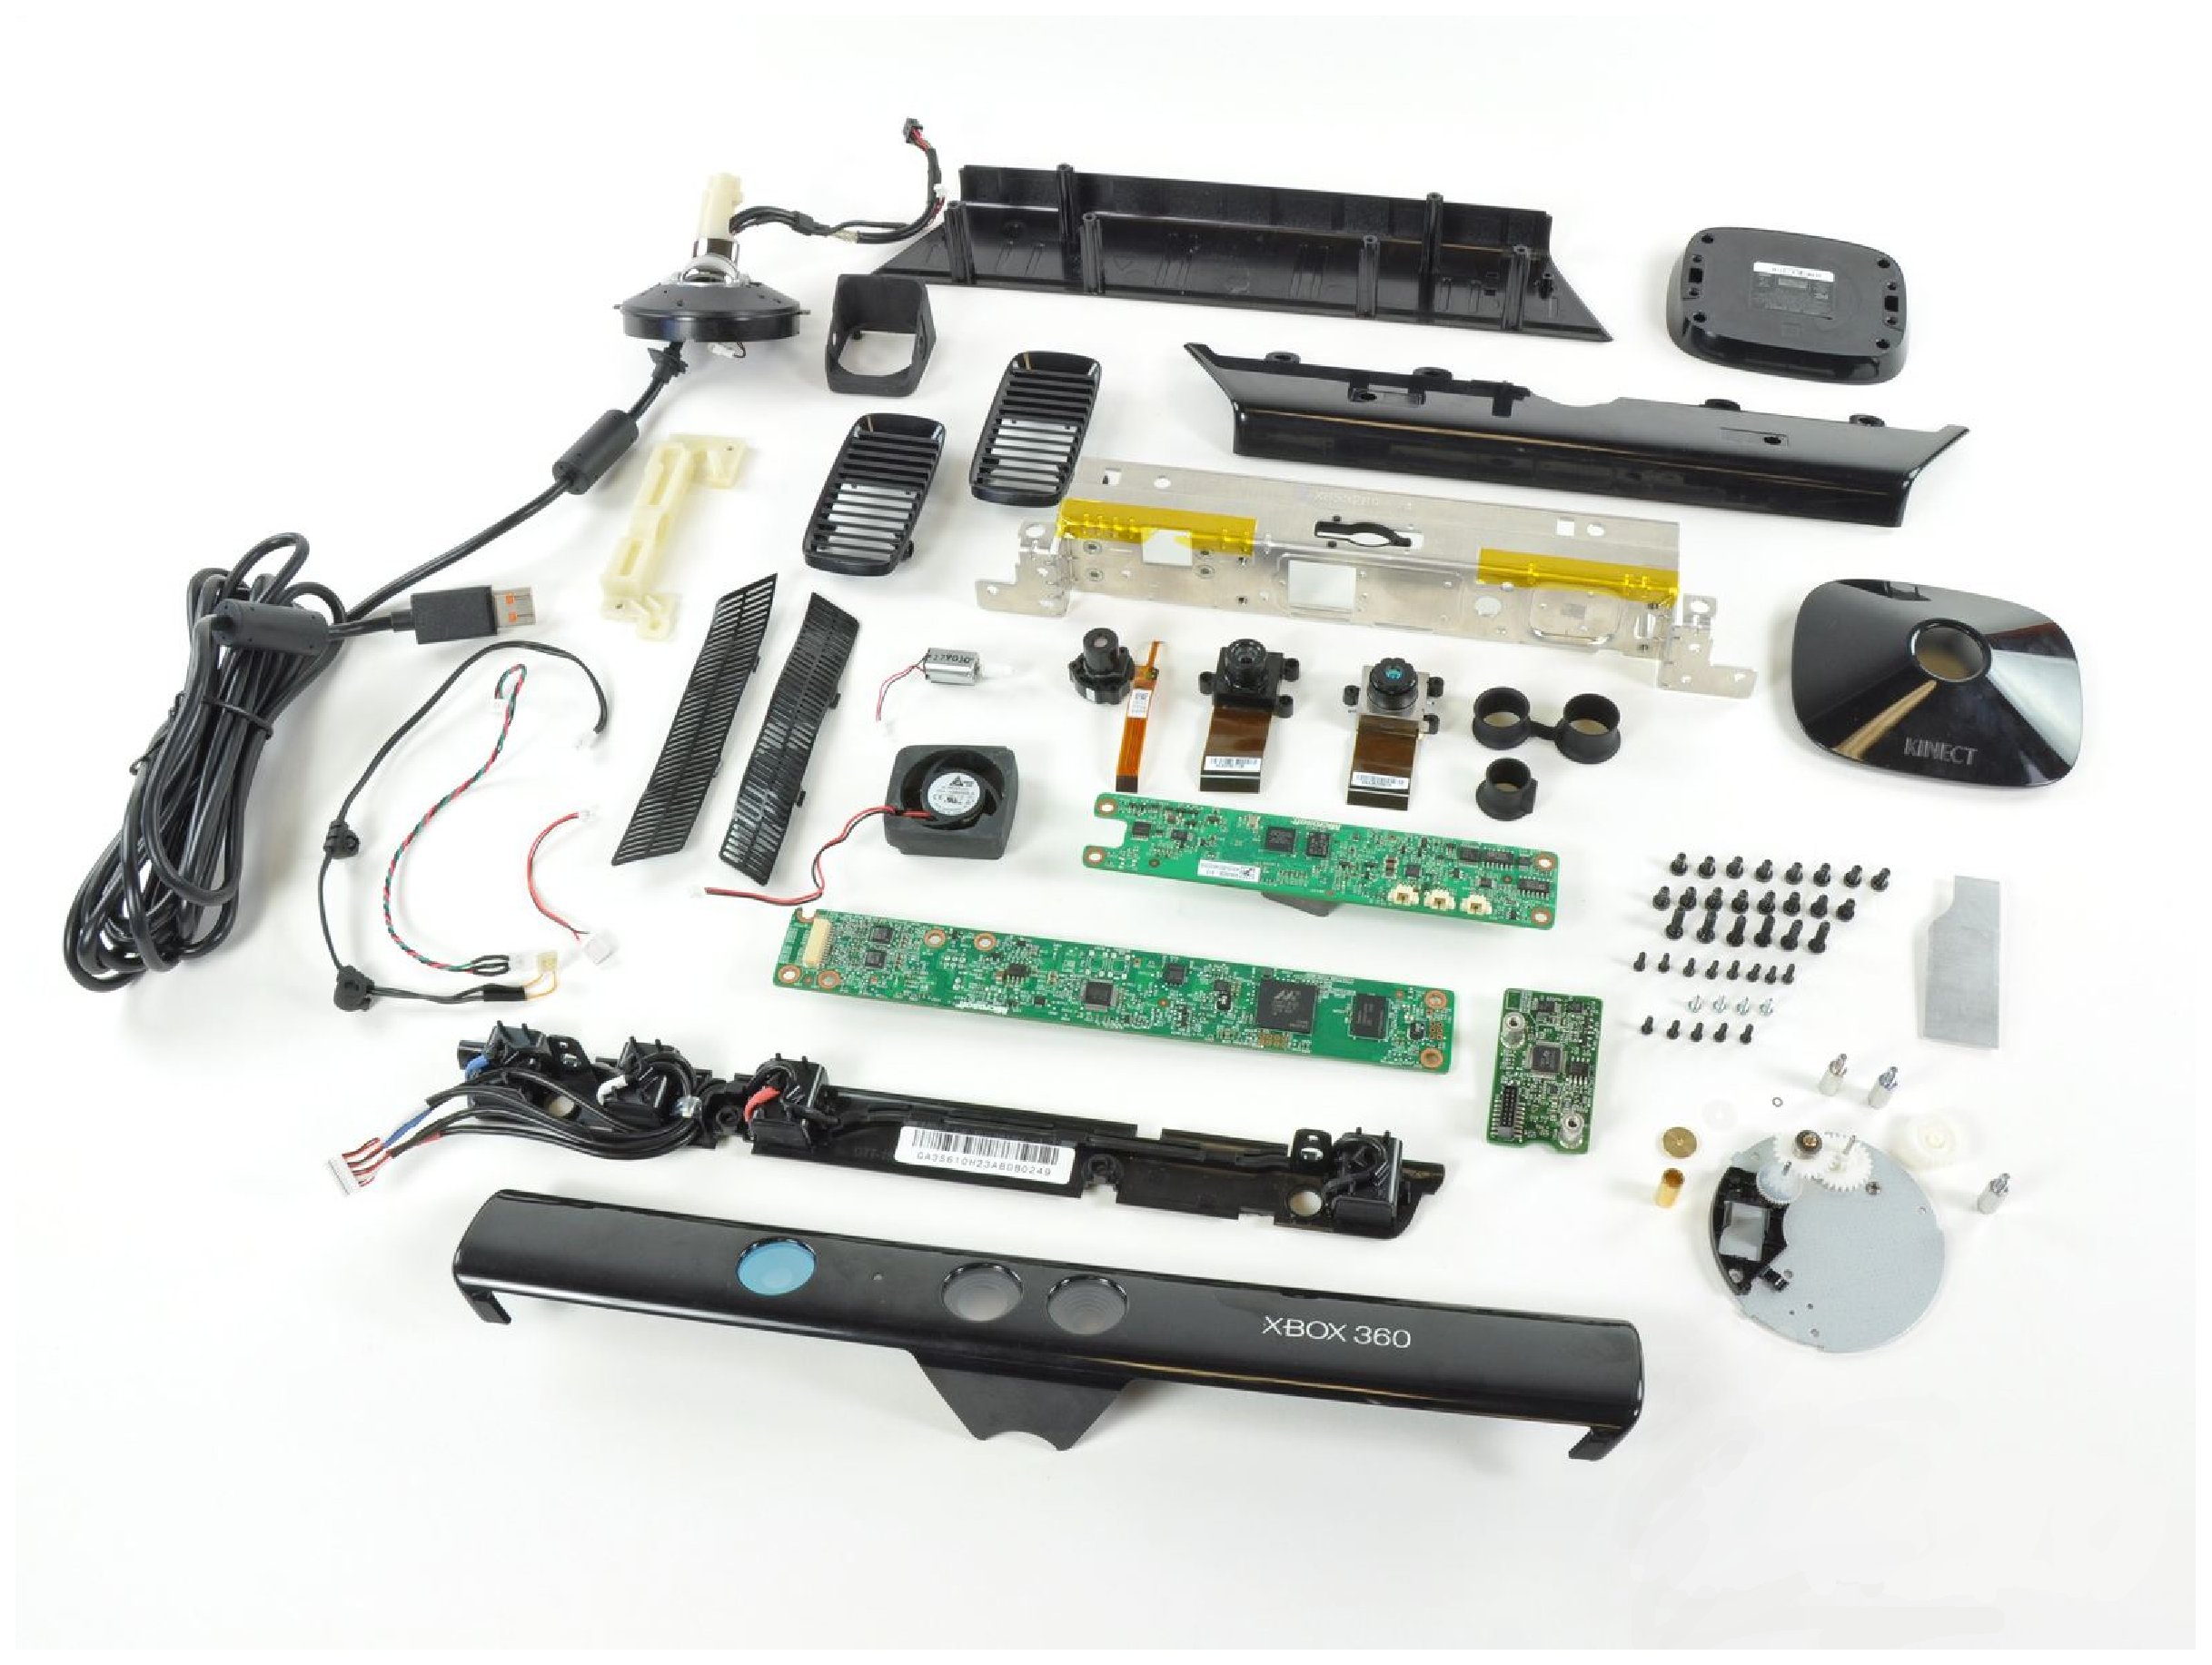
\includegraphics[scale=0.2]{img/kinect/kinect_parts.eps}
	\caption[Kinect Parts]{Kinect dismounted. Parts and components.}
	\end{center}

\end{figure}


%%%%%% The system's hardware %%%%%%
\addcontentsline{toc}{section}{The system's hardware}
\section{The system's hardware}

The hardware being used in this system is an RGB-D sensor. The information provided by this kind of device is more complete and makes the segmentation of the Region Of Interest easier. 
\\

Apart from that, there are various examples and libraries that allow an easy person tracking, showing its joints position in the 3-dimensional space. The 3D information allows a more precise, robust and noise-resistant joint location.
\\

Furthermore, the extra information handled permit a higher detail in the object recognition and learning nodes. Having two different algorithms running feature extraction and matching on different information makes a more robust description and recognition of the objects. 

